\documentclass[11pt,a4paper,3p,authoryear]{elsarticle}
\usepackage{geometry}
\geometry{a4paper,top=2.5cm,bottom=2.5cm,left=3cm,right=3cm}
\usepackage[utf8]{inputenc}
\usepackage[T1]{fontenc}
\usepackage{amsmath,amssymb,amsfonts}
\usepackage{graphicx}
\usepackage{booktabs}
\usepackage{lmodern}
\usepackage[expansion=false]{microtype}
\usepackage{siunitx}
\sisetup{per-mode=symbol,detect-all}
\DeclareSIUnit\calorie{cal}
\DeclareSIUnit\sol{sol}
\usepackage{multirow}
\bibliographystyle{elsarticle-harv}
\usepackage{hyperref}
\hypersetup{colorlinks=true, linkcolor=black, citecolor=black, urlcolor=blue}
\usepackage{cleveref}
\graphicspath{{../figures/}}
\journal{Preprint --- open release 2026}

\begin{document}

\begin{frontmatter}

\title{Crew time as the binding constraint of a bioregenerative food system for a fifteen-person, 500-sol Mars surface mission: design reconciliation and a 14-sol meal plan}

\author[a]{Mar\'ia Jes\'us Puerta Angulo\corref{cor1}}
\address[a]{Independent researcher, Tarragona, Spain}
\cortext[cor1]{Corresponding author. Email: \href{mailto:mariajesuspuertaangulo@gmail.com}{mariajesuspuertaangulo@gmail.com}}

\begin{abstract}
Bioregenerative food production is a candidate countermeasure for the NASA Human Research Program risk of inadequate food and nutrition on long-duration surface missions, but published architectures are seldom closed simultaneously against their lighting, water, thermal, atmospheric and crew-labour budgets. This paper reports the design of ESPERANZA~II, a food system sized for a crew of fifteen over a 500-sol (513.75 Earth-day) Mars surface rotation within a multi-rotation surface programme, developed for the 2026 NASA Mars to Table Challenge. The design premise follows from the challenge constraints: mass, power, volume and water are declared unconstrained, whereas crew time is bounded by a 45-hour workweek per five sols for each of two food specialists. The system comprises \SI{373}{\metre\squared} of LED sole-source crop canopy, a \SI{40}{\metre\squared} cyanobacterial photobioreactor, \SI{48}{\metre\squared} of \emph{Tenebrio molitor} rearing and \SI{50}{\metre\squared} of fungal culture, coupled to regolith processing and fermentation modules. Electrical demand is \SI{58.1}{\kilo\watt} mean and \SI{64.0}{\kilo\watt} peak; photoperiod tessellation holds canopy lighting peak within 9\,\% of its \SI{30.4}{\kilo\watt} mean. Canopy transpiration derived from absorbed light is \SI{644}{\litre} per sol, recovered at 98.5\,\%. Photosynthetic fixation of \SI{20.7}{\kilo\gram} CO$_2$ per sol exceeds crew respiration (\SI{15.4}{\kilo\gram}), with the deficit drawn from the Martian atmosphere; oxygen release is 116\,\% of crew demand. A 14-sol rotation of 78 distinct meals delivers \SI{3060}{\kilo\calorie} per crewmember per sol against a \SI{3035}{\kilo\calorie} target. Recomputation of all 1,004 ingredient operations of the rotation under a batch-processing protocol yields \SI{15.40}{\hour} of galley labour per sol (range 13.35--19.03) and a worst rolling five-sol window of \SI{80.3}{\hour} across the crew; the two specialists' load peaks at 79.5--\SI{81.2}{\hour} of the \SI{90}{\hour} budget, the range depending on whether grain milling is assigned to them or to the all-crew cooking rotation. Earth-provisioned energy is 41.2\,\% of menu calories on a per-ingredient audit (per-sol range 33.0--47.1\,\%) and 47.0\,\% on a conservative crop-nameplate basis, both below the 50\,\% cap; producing the EVA energy supplement in situ makes compliance independent of the EVA profile. Technology maturity ranges from TRL~3 (regolith mineral classification) to TRL~6--7 (LED crop production, fermentation). Workbooks and reconciliation scripts are released.
\end{abstract}

\begin{keyword}
bioregenerative life support \sep Mars surface mission \sep crew time \sep food system design \sep controlled-environment agriculture \sep in-situ resource utilisation \sep NASA Mars to Table
\end{keyword}

\end{frontmatter}

\section{Introduction}\label{sec:intro}

The NASA Human Research Program lists inadequate food and nutrition as a risk of performance decrement and crew illness on exploration missions \citep{NASAhrr2026}. For a Mars surface stay the risk is compounded by the shelf-life of pre-packaged food over mission durations of two to three years, by the absence of resupply, and by the psychological load of a fixed menu \citep{Douglas2020spacefood,Smith2021nutrition}. Bioregenerative food production---the cultivation of crops, microorganisms and other organisms within the habitat---has been studied as a countermeasure since the closed-ecosystem experiments of BIOS-3 \citep{Gitelson1989bios3}, the MELiSSA loop \citep{Lasseur2010melissa} and Lunar Palace~1 \citep{Fu2016lunarpalace}, and has flight heritage in small-scale hardware aboard the International Space Station \citep{Massa2017veggie}. Reviews of this work identify a recurring gap: crop productivities and radiation-use efficiencies are well characterised under controlled environments \citep{Wheeler2008productivity,Wheeler2017agriculture}, whereas system-level designs rarely reconcile lighting, water, heat rejection, atmospheric exchange and crew labour as one coupled budget \citep{Monje2003farming}.

The 2026 NASA Mars to Table Challenge \citep{NASAm2t2026} requested a complete food-system concept for a crew of fifteen over a 500-sol surface rotation, with a solution summary, a concept of operations, a 14-sol meal plan with per-ingredient lifecycle accounting, a design layout and a video walkthrough. The challenge rules state explicitly that mass, power, volume and water are \emph{not constrained}, and constrain one resource with mandatory language: all components of continuously maintaining the food system must be executable within a 45-hour workweek over five Martian sols for each of two specialists, without overtime. That asymmetry defines the design problem addressed here. Any production shortfall can be met with additional growing area, lighting and radiator surface at the cost of resources the rules do not ration; crew time is the one resource that cannot be expanded, and it therefore governs the architecture.

This paper documents the resulting system, ESPERANZA~II, and its reconciliation. The contributions are: (1) a system architecture in which crop, cyanobacterial, insect and fungal production lines are sized against a fixed crew-time budget rather than against mass or power; (2) resource ledgers for electrical power, lighting, water, carbon, oxygen and heat rejection that are closed against one another rather than against independent sources, a method which exposed and corrected a five-fold error in an earlier transpiration estimate; (3) a crew-time accounting method based on batch processing of ingredient events, recomputed here from the 1,004 ingredient lines of the delivered 14-sol meal plan and evaluated on rolling five-sol windows; (4) an Earth-provisioned energy audit on two declared bases together with a sensitivity analysis showing that in-situ production of the EVA energy supplement decouples rules compliance from the EVA schedule; and (5) a technology-maturity assessment that states the gaps to be closed for each element. \Cref{sec:mission} states the mission context and requirements, \cref{sec:arch} the architecture, \cref{sec:methods} the reconciliation methods, \cref{sec:results} the results, and \cref{sec:discussion} the discussion and limitations.

\section{Mission context and requirements}\label{sec:mission}

The design scenario is a relief crew of fifteen taking over a surface habitat and food system already in production, operating it for 500 sols and handing it over to the next crew during a 50-sol overlap. The system is required to sustain four or more consecutive rotations (approximately 5.6 Earth years) without mid-rotation cargo resupply; consumables are replenished by each incoming crew. \Cref{tab:req} lists the quantitative requirements taken from the challenge rules and from NASA-STD-3001.

\begin{table}[t]
\centering\small
\caption{Design requirements. Nutritional targets follow the spaceflight values of NASA-STD-3001 Vol.~2 \S7.1 \citep{NASAstd3001v2,Smith2021nutrition}; constraint language follows the challenge rules, Appendix~B \citep{NASAm2t2026}.}
\label{tab:req}
\begin{tabular}{@{}p{3.4cm}p{6.6cm}p{4.4cm}@{}}
\toprule
Parameter & Value & Source \\
\midrule
Crew & 15 & Rules \\
Surface rotation & 500 sols (513.75 Earth days) & Rules \\
Programme duration & $\geq 4$ rotations ($\approx 5.6$ yr) & Rules (multi-year objective) \\
Energy target & \SI{3035}{\kilo\calorie} per crewmember per sol & NASA-STD-3001 Vol.~2 \\
EVA supplement & +\SI{200}{\kilo\calorie} per crew-EVA-hour & Rules, p.~12 \\
Earth-provisioned food & $\leq 50\,\%$ of meal-plan calories & Rules, Appendix~B Table~3 \\
Crew time & $\leq \SI{45}{\hour}$ per 5 sols per specialist, 2 specialists, no overtime & Rules, Appendix~B (\emph{must}) \\
Mass, power, volume, water & Not constrained & Rules, Appendix~B \\
Habitat atmosphere & \SI{56.5}{\kilo\pascal} (8.2 psi), 34\,\% O$_2$, 18--\SI{27}{\celsius} & Rules \\
Surface gravity & \SI{3.71}{\metre\per\second\squared} & --- \\
Fire safety in hyperoxic volumes & Fire-rated enclosures, O$_2$ trim & NASA-STD-3001 Vol.~2 \S9.8.2 \\
\bottomrule
\end{tabular}
\end{table}

Two requirements interact in a way that shapes the design. The EVA supplement is meal-plan energy and is therefore subject to the 50\,\% cap; the cap must hold on every sol, not only on the rotation average. And because the crew-time requirement is assessed per specialist over a five-sol window, compliance depends on how galley labour is partitioned between the two specialists and the remaining thirteen crew, which the rules leave to the design.

\section{System architecture}\label{sec:arch}

\subsection{Production lines and growing area}

ESPERANZA~II produces food through four pathways occupying \SI{511}{\metre\squared} of growing area (\cref{tab:area}): a hydroponic crop canopy of eleven species under LED sole-source lighting; a cyanobacterial photobioreactor (\emph{Arthrospira platensis} for biomass, \emph{Anabaena} for nitrogen fixation at low partial pressure of N$_2$ \citep{Verseux2021cyano}); \emph{Tenebrio molitor} rearing on inedible crop biomass \citep{vanHuis2013insects}; and \emph{Pleurotus ostreatus} culture on crop residues. A galley, dining area, pantry, cold store and seed and culture bank occupy a further \SI{54}{\metre\squared}. The pressurised food-system volume is \SI{1058}{\metre\cubed}.

\begin{table}[t]
\centering\small
\caption{Growing and preparation areas. Only the crop canopy draws canopy lighting; photobioreactor illumination is internal to the cyanobacterial module, and the insect and fungal lines are heterotrophic.}
\label{tab:area}
\begin{tabular}{@{}p{7.4cm}S[table-format=3]p{5.4cm}@{}}
\toprule
Zone & {Area (m$^2$)} & Note \\
\midrule
Crop canopy, 11 species & 373 & Canopy LED, DLI 14--24 \si{\mole\per\metre\squared} per sol \\
Cyanobacterial photobioreactor & 40 & Illumination internal to module \\
\emph{Tenebrio molitor} racks & 48 & Heterotrophic \\
\emph{Pleurotus ostreatus} racks & 50 & Heterotrophic \\
\midrule
Total growing area & 511 & \\
Crew food deck (galley 14, dining 22, pantry 8, cold store 6, seed bank 4) & 54 & \\
\bottomrule
\end{tabular}
\end{table}

\Cref{tab:crops} gives the production nameplate by source, \SI{24141}{\kilo\calorie} per sol in total; four sources (wheat, \emph{Tenebrio}, \emph{Arthrospira}, potato) supply 83\,\% of fresh energy. Crop parameters follow the crop tables of the Life Support Baseline Values and Assumptions Document \citep{Anderson2018bvad}, which attributes them to the Kennedy Space Center Biomass Production Chamber and Utah State University work \citep{Wheeler2008productivity,Bugbee1997apogee}; the wheat figure uses the BVAD harvest index rather than the record yields of that literature.

\begin{table}[t]
\centering\small
\caption{Fresh production nameplate by source (steady state, sols 60--450). Percentages are of fresh energy. Yields are design values traced to \citet{Anderson2018bvad} (Tables 4-97, 4-105, 4-117, 4-119) and have not been confirmed at \SI{56.5}{\kilo\pascal} (\cref{sec:limitations}).}
\label{tab:crops}
\begin{tabular}{@{}lS[table-format=3]S[table-format=5]S[table-format=2.1]@{}}
\toprule
Source & {Area (m$^2$)} & {kcal per sol} & {\% fresh} \\
\midrule
Wheat & 150 & 6027 & 25.0 \\
\emph{Arthrospira} (photobioreactor) & 40 & 5800 & 24.0 \\
\emph{Tenebrio molitor} (racks) & 48 & 5600 & 23.2 \\
Potato & 80 & 2640 & 10.9 \\
Soybean & 80 & 1784 & 7.4 \\
\emph{Pleurotus} (racks) & 50 & 1375 & 5.7 \\
Radish & 8 & 307 & 1.3 \\
Lettuce and kale & 15 & 248 & 1.0 \\
Tomato & 20 & 144 & 0.6 \\
Pepper & 15 & 130 & 0.5 \\
Herbs & 5 & 86 & 0.4 \\
\midrule
Total & 511 & 24141 & 100.0 \\
\bottomrule
\end{tabular}
\end{table}

The crop chambers hold an atmosphere independent of the habitat: \SI{56.5}{\kilo\pascal} total pressure, approximately 21\,\% O$_2$ and 1,200--1,500 ppm CO$_2$, airlock-separated and exporting O$_2$ to the habitat. All staple crops (wheat, soybean, potato, tomato, pepper) are C$_3$ species; at the habitat's 34\,\% O$_2$ the oxygenase reaction of Rubisco competes more strongly with carboxylation and net photosynthesis falls by an estimated 15--25\,\%, which would render the crop-table yields optimistic. LED driver electronics are housed in a normoxic bay with DC distribution to the luminaires.

\subsection{Regolith processing and substrate}

Three modules process Martian regolith into a growth substrate. A regolith mineral classifier (random forest and Gaussian-process regression trained on published lunar and Martian compositional datasets; TRL~3) ranks candidate feedstock. A perchlorate bioremediation stage uses perchlorate-reducing bacteria of the \emph{Azospira} group, whose \emph{pcrA}/\emph{cld} pathway is characterised \citep{Melnyk2011perchlorate}, to reduce perchlorate from the 0.4--0.6 wt\,\% measured at the Phoenix site \citep{Hecht2009perchlorate} to a design gate of 0.017 wt\,\% by sol~24 of the substrate cycle; the acceptance criterion for crop tissue is the U.S.\ EPA reference dose of \SI{0.7}{\micro\gram\per\kilo\gram} per day \citep{EPA2005perchlorate}. Perchlorate is treated as a hazard to be removed rather than as an oxygen resource \citep{Davila2013perchlorate}: chlorite dismutase generates O$_2$ intracellularly and the organism respires it in situ, so no oxygen from this stage is credited to the atmospheric balance. The substrate is a blend of 32.1\,\% lunar regolith (transported as transit radiation shielding and repurposed as a calcium and magnesium corrector), 21.3\,\% treated Martian regolith, 20\,\% cyanobacterial biomass, 24.4\,\% composted organics and 2.2\,\% biopolymer binder; the rationale for regolith-based substrates follows the reviews of \citet{Duri2022regolith} and \citet{Fackrell2024regolith}.

\subsection{Fermentation and operations layer}

A fermentation module produces miso, tempeh, kefir, bread and vinegar and hosts the insect line. An operations layer (NEXUS) aggregates approximately 200 sensors across the modules, schedules galley and cultivation tasks, and proposes per-crewmember portioning from non-invasive wearable data; it proposes and the crew decides, and the nutritional targets of the meal plan are met in full if the layer is ignored. The inference step on which its state detection rests was demonstrated by the author on public NASA flight data \citep{PuertaAngulo2026hrp} and is discussed in \cref{sec:discussion}.

\section{Methods}\label{sec:methods}

\subsection{Reconciliation principle}

Every budget was closed against its neighbours rather than against an independent source. The lighting power that drives the electrical budget is the same energy that drives canopy transpiration and heat rejection; the ingredient list that drives the Earth-provisioned fraction is the same list that drives galley labour. This principle is stated first because it is how the largest error in the design history was found (\cref{sec:water}).

\subsection{Lighting and electrical power}

Canopy lighting power is computed from the daily light integral $D_i$ (\si{\mole\per\metre\squared} per sol) and area $A_i$ of each crop zone $i$, the fixture efficacy $\eta$ (\si{\micro\mole\per\joule}) and the sol length $t_\mathrm{sol} = \SI{88775}{\second}$:
\begin{equation}
P_\mathrm{LED,mean} = \frac{\sum_i D_i A_i}{\eta\, t_\mathrm{sol}}, \qquad
P_\mathrm{LED}(t) = \sum_i \frac{D_i A_i}{\eta\, \tau_i}\,\mathbb{1}[t \in W_i],
\label{eq:led}
\end{equation}
where $\tau_i$ is the photoperiod of zone $i$, $W_i$ its lit window within the sol and $\mathbb{1}[\cdot]$ the indicator function (1 when the zone is lit, 0 otherwise). The efficacy is taken as $\eta = 3.0$ \si{\micro\mole\per\joule}, achievable in current commercial horticultural fixtures at the favourable end of the range; a sensitivity at 2.7 \si{\micro\mole\per\joule} is reported. Photoperiods are crop-physiology requirements first: soybean is a short-day species that does not flower under 16-hour days, and potato tuberisation favours short days, so both run on 12.33-hour windows; wheat (cv.\ USU-Apogee, bred for controlled environments and tolerant of continuous light \citep{Bugbee1997apogee}) runs 24/0. The remaining electrical line items (ventilation with hypobaric density correction, dehumidification, thermal-loop pumping, nutrient pumps, substrate pasteurisation, galley, cold store, CO$_2$ capture) are estimated from stated bases (\cref{tab:power}).

\subsection{Water}\label{sec:water}

In a closed chamber the energy for evapotranspiration can only come from absorbed light. Gross canopy transpiration is therefore derived from the lighting budget:
\begin{equation}
E = \frac{P_\mathrm{LED,mean}\, f_\mathrm{abs}\, f_\mathrm{lat}\, t_\mathrm{sol}}{L_v},
\label{eq:transp}
\end{equation}
with absorbed fraction $f_\mathrm{abs} = 0.90$, latent partition $f_\mathrm{lat} = 0.65$ and latent heat of vaporisation $L_v = \SI{2450}{\kilo\joule\per\kilo\gram}$. An earlier revision of the design carried \SI{3226}{\litre} per sol of transpiration; evaporating that mass requires \SI{89}{\kilo\watt} of latent heat against \SI{30.4}{\kilo\watt} of lighting, and the figure, together with a \SI{50}{\litre} per sol in-situ water input that had been sized to it, was withdrawn. Condensate recovery at chamber condensers is taken as 98.5\,\%; make-up is drawn from habitat grey water. Condenser control uses hot-gas bypass with a 4--\SI{10}{\celsius} setpoint and a trip below \SI{2}{\celsius} to avoid icing against a loop near Martian ambient.

\subsection{Carbon and oxygen}

CO$_2$ fixation by the canopy is computed from dry-matter production ($\SI{23.5}{\gram\per\metre\squared}$ per sol over \SI{373}{\metre\squared}, i.e.\ \SI{8.77}{\kilo\gram} dry biomass per sol, 307 mol C) and by the photobioreactor from its biomass yield; O$_2$ release follows photosynthetic stoichiometry (32/44 by mass). Crew respiration and oxygen demand use the baseline values of \citet{Anderson2018bvad}. Fermentation, composting and heterotrophic lines return CO$_2$ to the canopy; any residual deficit is met by capture and compression of Martian atmospheric CO$_2$ (0.6 to \SI{56.5}{\kilo\pascal}, 94:1).

\subsection{Heat rejection}

Essentially all electrical input becomes heat, less the fraction stored as chemical energy in biomass: $Q = P_\mathrm{el} - P_\mathrm{chem}$. The radiator is sized for the dust-deposited case (solar absorptivity $\alpha \approx 0.55$) rather than the clean case ($\alpha \approx 0.15$), at a \SI{40}{\celsius} loop with vertical north--south panels; the cleaning cadence is set by the same deposition rate and its EVA hours are charged to the calorie budget at \SI{200}{\kilo\calorie} per crew-EVA-hour. Global dust storms, which suppress surface photosynthetically active radiation by more than 90\,\% for weeks without reliable forecast \citep{Zurek1993duststorms}, are the first of three grounds on which conducted daylight was traded out of the lighting architecture; the others are pressure-shell penetrations and the conductive loss of a translucent boundary (15--\SI{46}{\kilo\watt} over \SI{373}{\metre\squared} at $\Delta T \approx \SI{82}{\kelvin}$ for $U = 0.5$--\SI{1.5}{\watt\per\metre\squared\per\kelvin}, against roughly \SI{17}{\kilo\watt} of optical gain).

\subsection{Crew-time accounting}\label{sec:crewtime-method}

The delivered meal-lifecycle workbook records, for each of the 1,004 ingredient lines of the 14-sol rotation, a preparation, cooking and cleaning duration. Durations are charged per ingredient \emph{event} under a batch-processing (mise en place) galley protocol: preparation once per ingredient per sol, cooking once per ingredient per meal, cleaning once per ingredient per sol; subsequent lines of the same ingredient within the batching scope carry zero. The unbatched line-by-line sum is retained as a reference because it double-charges mise en place for ingredients recurring across a sol's services (soybean oil alone appears on 130 lines).

For this paper the per-sol galley load $G_s$ was recomputed directly from the workbook as the sum of the three duration columns over all lines served on sol $s$ (script \texttt{01\_recompute\_from\_deliverables.py}), and evaluated on the ten distinct rolling five-sol windows of the rotation, $\sum_{k=0}^{4} G_{s+k}$ for $s = 1,\dots,10$. Compliance is assessed on the two specialists' own load. Galley work is partitioned by activity: in-situ ingredient processing (fermentation, spirulina harvest, insect and mushroom handling, soy and grain processing) is retained by the specialists; Earth-ingredient preparation, cooking and galley cleaning are carried by an all-crew cooking rotation. Specialist non-galley duties (crop tending and harvest, HACCP and water and perchlorate monitoring, maintenance, documentation, planning) are added. The non-galley durations are design allocations stated in the concept of operations and are not recomputed here. The activity partition is examined two ways: as the design allocation (\SI{28.1}{\hour} per cycle retained by the specialists), and as a recomputation that classifies each workbook line by its \emph{Production Method} field into in-situ processing (fermentation, insect, fungal, soy-processing and photobioreactor lines), crop preparation (hydroponic crop lines) and Earth stock, and sums the specialists' in-situ processing hours on the same rolling windows. The workbook does not separate grain milling from crop preparation, so the recomputation is a lower bound on the specialists' galley share and the design allocation an upper bound.

\subsection{Earth-provisioned energy audit}\label{sec:audit-method}

The rules specify the Earth-provisioned fraction by calories, but the lifecycle workbook records source and mass without energy and the schedule workbook records energy without source. Each of the 177 distinct ingredient labels was therefore assigned an energy density from a named USDA FoodData Central reference item \citep{USDAfdc}, volumetric entries were converted to mass (cooking oil at \SI{0.92}{\gram\per\milli\litre}; all other volumetric entries at unity), and line energy was aggregated by source and by sol. A confidence class (high, medium, low) was recorded per label. The audit was validated by reconstructing the plan's own energy without fitting: \SI{2992}{\kilo\calorie} per crewmember per sol against the \SI{3035}{\kilo\calorie} target (98.6\,\%). Two bases are reported: the audited menu, and a conservative crop-nameplate basis in which the in-situ line is fixed at the crop-table production of \SI{24141}{\kilo\calorie} per sol and any menu draw above it is booked to Earth stock as a declared reserve.

\subsection{Reproducibility}

The recomputation used Python~3 with \texttt{openpyxl} and \texttt{matplotlib}; it is deterministic and completes in seconds. The delivered workbooks are read unmodified; results are written to \texttt{results.json} and \texttt{per\_sol.csv}. Figures are generated by \texttt{02\_figures.py}. The lighting, water, gas, heat and EVA computations use the closed-form expressions above with the stated constants.

\section{Results}\label{sec:results}

\subsection{Electrical power}

Food-system demand is \SI{58.1}{\kilo\watt} mean, \SI{64.0}{\kilo\watt} peak and \SI{77}{\kilo\watt} installed (peak $\times 1.20$). \Cref{tab:power} gives the ledger. Canopy lighting is 52\,\% of the mean. At $\eta = 2.7$ \si{\micro\mole\per\joule} canopy demand rises to approximately \SI{33.8}{\kilo\watt} mean, within the installed capacity without redesign.

\begin{table}[t]
\centering\small
\caption{Electrical power ledger (mean, kW). Photobioreactor illumination, mixing and sparging are internal to the cyanobacterial module and are not part of the canopy figure; insect rearing is internal to the fermentation module.}
\label{tab:power}
\begin{tabular}{@{}p{5.4cm}S[table-format=2.1]p{7.6cm}@{}}
\toprule
Line item & {kW} & Basis of estimate \\
\midrule
Six process modules & 10.7 & Classifier 0.6, bioremediation 2.1, substrate 0.4, cyanobacteria 4.8, fermentation 1.9, operations layer 0.9 \\
Canopy LED & 30.4 & \Cref{eq:led}, \SI{373}{\metre\squared} \\
Canopy ventilation & 5.0 & 8\,\% of lighting load $\times$ 1.84 hypobaric correction ($\rho$ 0.667 vs \SI{1.225}{\kilo\gram\per\metre\cubed}) \\
Dehumidification and condensate & 2.2 & \SI{17.8}{\kilo\watt} latent rejected passively; pumping only \\
Thermal loop and pumps & 2.5 & $\approx 4\,\%$ of rejected thermal load \\
Nutrient and aeration pumps & 2.5 & 5--\SI{8}{\watt\per\metre\squared} hydroponic practice \\
Substrate pasteurisation & 1.2 & Batch, sol-averaged \\
Work and corridor lighting & 0.8 & Task and egress illumination \\
Galley (mill, griddle, centrifuge) & 0.7 & Equipment inventory \\
Mushroom chamber environment & 0.6 & 90\,\% RH, elevated air change \\
Refrigerated store, \SI{4}{\celsius} & 0.8 & Storage condition of the meal plan \\
Water treatment and condensate UV & 0.4 & Potable polishing \\
CO$_2$ capture and compression & 0.3 & \SI{3.1}{\kilo\gram} per sol; isothermal ideal work \SI{8.8}{\watt}, $\sim 7\times$ margin \\
\midrule
Total, mean & 58.1 & Peak 64.0; installed 77 \\
\bottomrule
\end{tabular}
\end{table}

\subsection{Lighting and photoperiod tessellation}

\Cref{tab:zones} and \cref{fig:led} show the canopy zones and the instantaneous load over one sol. Wheat runs as a continuous baseload; soybean and potato occupy opposite 12.33-hour windows; fruiting and leafy crops run 16/8. The resulting peak of \SI{33.3}{\kilo\watt} sits 9\,\% above the \SI{30.4}{\kilo\watt} mean, which is what allows a power plant of modest class to serve a \SI{373}{\metre\squared} farm without a large battery.

\begin{table}[t]
\centering\small
\caption{Canopy zones, daily light integral (DLI), photoperiod and lighting load. Instantaneous load applies while the zone is lit.}
\label{tab:zones}
\begin{tabular}{@{}lS[table-format=3]S[table-format=2]lS[table-format=2.2]S[table-format=2.2]@{}}
\toprule
Zone & {Area (m$^2$)} & {DLI} & Photoperiod (h) & {Instantaneous (kW)} & {Mean (kW)} \\
\midrule
Wheat, USU-Apogee & 150 & 24 & 24/0 & 13.52 & 13.52 \\
Soybean & 80 & 22 & 12.33/12.33 & 13.22 & 6.61 \\
Potato & 80 & 20 & 12.33/12.33, opposite & 12.02 & 6.01 \\
Tomato, pepper, leafy greens & 63 & {14--22} & 16/8 & 6.55 & 4.25 \\
\midrule
Canopy & 373 & & & 33.3 & 30.4 \\
\bottomrule
\end{tabular}
\end{table}

\begin{figure}[t]
\centering
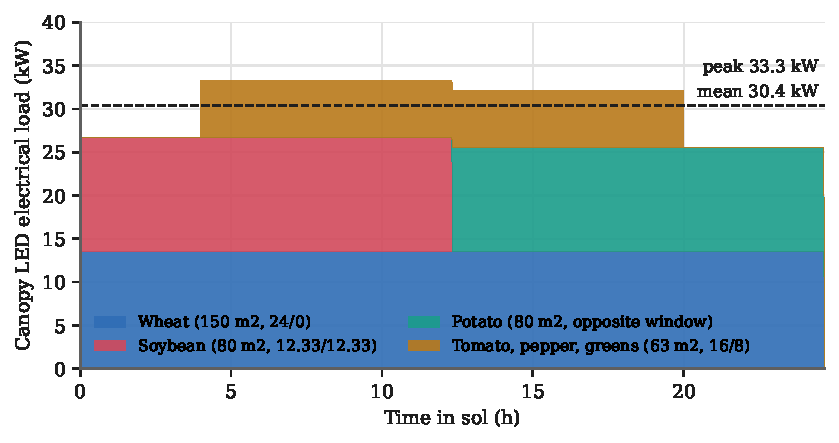
\includegraphics[width=\linewidth]{fig1_led_photoperiod.pdf}
\caption{Canopy LED electrical load over one sol (24.66 h) by crop zone, stacked. Wheat (\SI{150}{\metre\squared}) runs continuously; soybean and potato (\SI{80}{\metre\squared} each) occupy opposite 12.33-hour windows; fruiting and leafy crops (\SI{63}{\metre\squared}) run 16/8. The dashed line is the sol mean (\SI{30.4}{\kilo\watt}); the peak is \SI{33.3}{\kilo\watt}. Zone loads from \cref{tab:zones}.}
\label{fig:led}
\end{figure}

\subsection{Water}

\Cref{tab:water} gives the water streams. Gross canopy transpiration from \cref{eq:transp} is \SI{644}{\litre} per sol, of which \SI{634}{\litre} is recovered as condensate; net make-up is \SI{9.7}{\litre} per sol, supplied from the \SI{12}{\litre} per sol of grey water received from the habitat ECLSS. The \SI{12000}{\litre} nutrient-solution inventory (\SI{32}{\litre\per\metre\squared}) is inherited with the habitat and is not a daily flow. The food system does not generate water; it conserves it, and initial water procurement lies outside its boundary.

\begin{table}[t]
\centering\small
\caption{Water streams (per sol). The transpiration figure is derived from the lighting budget (\cref{eq:transp}) and replaces a withdrawn earlier estimate of \SI{3226}{\litre} per sol.}
\label{tab:water}
\begin{tabular}{@{}p{5.2cm}S[table-format=5.1]p{7.6cm}@{}}
\toprule
Stream & {L per sol} & Basis \\
\midrule
Canopy transpiration, gross & 644 & \SI{30.4}{\kilo\watt} $\times$ 0.90 $\times$ 0.65 / \SI{2450}{\kilo\joule\per\kilo\gram} \\
Condensate recovered & 634.3 & 98.5\,\% recovery \\
Net make-up & 9.7 & 644 $\times$ 1.5\,\% \\
Grey water received from ECLSS & 12 & Habitat interface \\
Nutrient solution inventory & 12000 & Standing volume, not a flow \\
\bottomrule
\end{tabular}
\end{table}

\subsection{Carbon and oxygen}

\Cref{tab:gas} and \cref{fig:gas} give the ledger. The canopy fixes \SI{13.5}{\kilo\gram} CO$_2$ per sol and the photobioreactor \SI{7.2}{\kilo\gram}, a total of \SI{20.7}{\kilo\gram}. Crew respiration supplies \SI{15.4}{\kilo\gram} (74\,\%); fermentation, composting and heterotrophic lines return \SI{2.8}{\kilo\gram}; the remaining \SI{2.5}{\kilo\gram} is drawn from the Martian atmosphere (\SI{3.1}{\kilo\gram} captured, \SI{0.6}{\kilo\gram} buffered). Fifteen crew are not a sufficient carbon source to saturate \SI{413}{\metre\squared} of photosynthetic area; the loop is closed on the resources that are scarce (water, organics) and deliberately open on the one that is abundant outside the habitat. Oxygen release is \SI{9.82}{\kilo\gram} per sol from crops and \SI{5.20}{\kilo\gram} from the photobioreactor, \SI{15.02}{\kilo\gram} in total against a crew demand of \SI{12.95}{\kilo\gram} (116\,\%); crops alone supply 76\,\%.

\begin{table}[t]
\centering\small
\caption{Carbon and oxygen ledger (kg per sol). Crew values from \citet{Anderson2018bvad}. No oxygen from perchlorate reduction is credited.}
\label{tab:gas}
\begin{tabular}{@{}p{6.4cm}S[table-format=2.2]p{6.4cm}@{}}
\toprule
Stream & {kg per sol} & Basis \\
\midrule
CO$_2$ fixed by crops & 13.5 & 307 mol C; \SI{8.77}{\kilo\gram} dry biomass \\
CO$_2$ fixed by photobioreactor & 7.2 & 35\,\% of total fixation \\
CO$_2$ from crew respiration & 15.4 & Metabolic baseline \\
CO$_2$ from fermentation, composting, heterotrophs & 2.8 & 1.5 + 0.8 + 0.5 \\
CO$_2$ captured from Martian atmosphere & 3.1 & 0.6 buffered; 2.5 net \\
O$_2$ released by crops & 9.82 & Stoichiometry from 13.5 kg CO$_2$ \\
O$_2$ released by photobioreactor & 5.20 & Stoichiometry from 7.2 kg CO$_2$ \\
O$_2$ consumed by crew & 12.95 & Metabolic baseline \\
\midrule
Total O$_2$ released & 15.02 & 116\,\% of demand \\
\bottomrule
\end{tabular}
\end{table}

\begin{figure}[t]
\centering
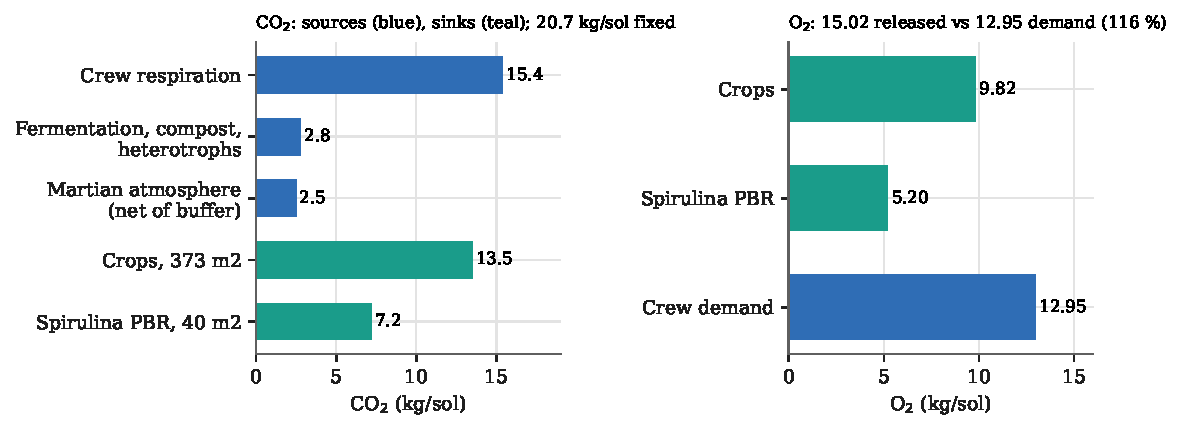
\includegraphics[width=\linewidth]{fig4_gas_ledger.pdf}
\caption{Carbon and oxygen ledger per sol. Left: CO$_2$ sources (crew, heterotrophic returns, Martian atmosphere net of buffer) and sinks (crop canopy, photobioreactor). Right: O$_2$ released by the two photosynthetic lines against crew demand. Values as stated in the design documents (\cref{tab:gas}); not recomputed.}
\label{fig:gas}
\end{figure}

\subsection{Heat rejection}

Thermal load to reject is \SI{58.1}{\kilo\watt} electrical less \SI{1.7}{\kilo\watt} stored in biomass, i.e.\ \SI{56.4}{\kilo\watt}. A clean radiator at mean conditions requires approximately \SI{220}{\metre\squared}; under dust deposition a \SI{230}{\metre\squared} array fails to reject at local noon. The array is therefore sized at approximately \SI{300}{\metre\squared}, at a \SI{40}{\celsius} loop, with vertical north--south panels and a scheduled cleaning EVA (2 crew $\times$ \SI{4}{\hour} every 30 sols, 0.27 crew-EVA-hours per sol). Together with regolith acquisition for the substrate (\SI{10.5}{\kilo\gram} of Martian regolith per sol, batched as 2 crew $\times$ \SI{6}{\hour} every 30 sols, 0.40 crew-EVA-hours per sol), the EVA demand attributable to the food system is 0.7 crew-EVA-hours per sol, one twelfth of the 8 crew-EVA-hours per sol nominal mission envelope.

\subsection{Crew time}\label{sec:crewtime-results}

Recomputed from the 1,004 ingredient lines, galley labour across the whole crew is \SI{15.40}{\hour} per sol on average (preparation 6.55, cooking 6.23, cleaning \SI{2.62}{\hour}), with a peak of \SI{19.03}{\hour} on sol~3, a second peak of \SI{18.72}{\hour} on sol~13 and a minimum of \SI{13.35}{\hour} on sol~6 (\cref{fig:crew}, left). The rotation totals \SI{76.98}{\hour} per five sols on average; the worst of the ten rolling five-sol windows (sols 10--14) totals \SI{80.27}{\hour} (\cref{fig:crew}, right). The unbatched line-by-line sum is \SI{21.03}{\hour} per sol, 37\,\% higher, which quantifies the labour value of the batch protocol.

Under the activity partition of \cref{sec:crewtime-method}, the all-crew cooking rotation carries \SI{48.9}{\hour} per cycle (Earth-ingredient preparation 4.7, cooking 31.2, galley cleaning \SI{13.1}{\hour}; approximately \SI{45}{\minute} per person per sol across thirteen crew) and the two specialists retain \SI{28.1}{\hour} per cycle of in-situ ingredient processing. With \SI{49.0}{\hour} per cycle of non-galley duties (crop tending and harvest 22.0, HACCP and water and perchlorate monitoring 9.0, maintenance 7.0, documentation 6.0, planning and inventory \SI{5.0}{\hour}), the specialists' mean load is \SI{77.1}{\hour} of \SI{90}{\hour} (86\,\%), the worst window \SI{81.2}{\hour} (90\,\%), the worst single specialist \SI{40.6}{\hour} of 45, and none of the ten windows exceeds the budget. Without the cooking rotation the specialists would require \SI{126}{\hour} per cycle. No specialist sol exceeds \SI{9}{\hour}; the binding criterion is the five-sol window, not any single sol.

The recomputed partition by production method gives \SI{23.8}{\hour} per cycle of in-situ processing, \SI{36.2}{\hour} of crop preparation and \SI{17.0}{\hour} of Earth-stock handling (sum \SI{77.0}{\hour}). In-situ processing peaks at \SI{30.5}{\hour} in its worst five-sol window (sols 2--6, driven by fermentation batches on sols 2 and 3), which with the \SI{49.0}{\hour} of non-galley duties gives a specialist load of \SI{79.5}{\hour} (88\,\%) in the worst window and \SI{72.8}{\hour} (81\,\%) on average. The design allocation, which additionally assigns grain milling to the specialists, gives \SI{81.2}{\hour}; the two bases bracket the specialists' worst window at 79.5--\SI{81.2}{\hour}, and both satisfy the \SI{90}{\hour} requirement with 9--11\,\% margin.

\begin{figure}[t]
\centering
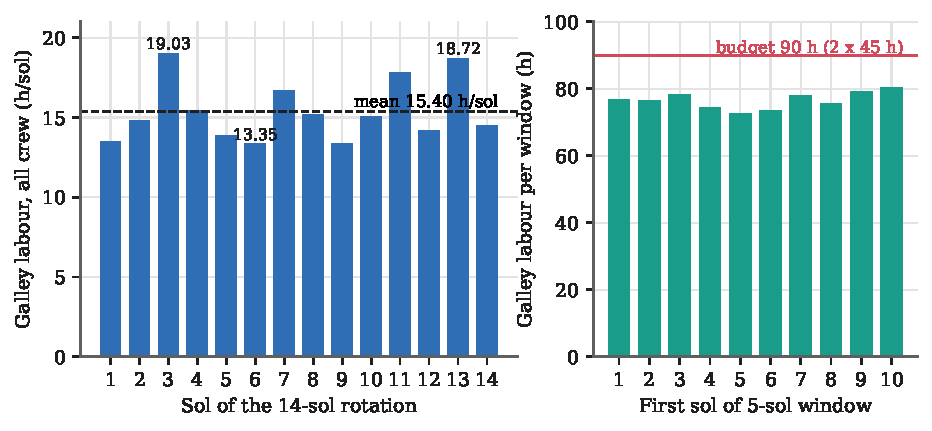
\includegraphics[width=\linewidth]{fig2_crew_time.pdf}
\caption{Galley labour recomputed from the delivered 14-sol meal plan (1,004 ingredient lines, batch protocol). Left: hours per sol across the whole crew; dashed line, rotation mean \SI{15.40}{\hour}; labelled sols are the two peaks and the minimum. Right: labour in each of the ten rolling five-sol windows against the \SI{90}{\hour} two-specialist budget; the worst window (sols 10--14) totals \SI{80.3}{\hour} before partition between specialists and the all-crew cooking rotation.}
\label{fig:crew}
\end{figure}

\subsection{Meal plan and nutrition}

The rotation comprises 78 distinct meals (no meal repeated within 14 sols) drawn from 12 food sources and 16 species or cultured organisms, with six primary protein sources (\emph{Tenebrio}, soybean products, chickpea, \emph{Arthrospira}, wheat gluten, \emph{Pleurotus}). Recomputed from the schedule workbook, delivered energy is \SI{3059.9}{\kilo\calorie} per crewmember per sol on average (100.8\,\% of target; range 3035--3257), protein \SI{123.1}{\gram} (target 91), fibre \SI{57.7}{\gram} (target 30) and sodium \SI{1852.5}{\milli\gram} (limit 2,300); carbohydrate is \SI{423}{\gram} (target 380) and fat \SI{94.2}{\gram} (93.3\,\% of target, 27.7\,\% of energy). Protein and fibre run above target by design, the former in support of bone and muscle countermeasures and the latter to feed short-chain fatty acid production \citep{Turroni2020microbiome,QuinnBohmann2024mcmm}. Micronutrient values are design estimates at 70\,\% yield derating rather than an audited roll-up: vitamin D follows the \SI{25}{\micro\gram} per sol spaceflight requirement (\SI{18}{\micro\gram} from UV-treated \emph{Pleurotus}, \SI{7}{\micro\gram} from an Earth-provisioned premix); iodine (\SI{150}{\micro\gram}) is supplied entirely by the premix because perchlorate competitively inhibits thyroidal iodide uptake, and compliance is verified by urinary iodine and TSH every 90 sols; iron from whole foods is \SI{20}{\milli\gram} per sol against the spaceflight ceiling of 8--\SI{10}{\milli\gram} \citep{Smith2021nutrition}, an open non-conformance discussed in \cref{sec:limitations}. Fermented foods carrying live cultures (kefir, miso, tempeh) are embedded in the rotation rather than supplied as supplements, following the rationale reviewed by \citet{Zhao2024polyphenols}.

\subsection{Earth-provisioned fraction and EVA sensitivity}

On the per-ingredient audit the 14-sol menu supplies \SI{24619}{\kilo\calorie} per crewmember from in-situ production and \SI{17258}{\kilo\calorie} from Earth stock, an Earth-provisioned fraction of 41.2\,\%, with a per-sol range of 33.0--47.1\,\% (\cref{fig:earth}, left); no sol exceeds the cap. On the crop-nameplate basis the fraction is 47.0\,\%: the menu draws \SI{2628}{\kilo\calorie} per sol above the \SI{24141}{\kilo\calorie} per sol crop table and that draw is booked to Earth stock. The higher figure is carried as the headline. Of the 177 ingredient labels, 62 are high-confidence, 57 medium and 58 low; weighted by contribution, 67\,\% of calories come from high-confidence entries and 6.4\,\% from low-confidence entries, the latter dominated by spice blends of 1--\SI{3}{\gram}. Cooking oil is 3\,\% of ingredient mass but 15\,\% of plan energy and is Earth-provisioned; it is the dominant lever on the audited fraction. For reference, the same audit by mass yields 16.1\,\%; mass is not the metric the rules specify.

The EVA energy supplement is meal-plan energy and is subject to the cap. \Cref{tab:eva} and \cref{fig:earth} (right) show the fraction on the nameplate basis as a function of crew EVA hours per sol under two sourcing options. Supplied from Earth, the cap is breached at 13.8 crew-EVA-hours per sol, a cadence set by the surface architecture rather than by the food system. Produced in situ, the fraction decreases monotonically with EVA hours, from 47.0\,\% at zero to 42.5\,\% at the 24-hour design box; at the nominal 8 crew-EVA-hours per sol it is 45.4\,\%. The in-situ option costs \SI{25}{\metre\squared} of additional canopy, \SI{2.0}{\kilo\watt} of LED, \SI{13}{\metre\squared} of radiator and \SI{0.6}{\litre} per sol of make-up water, moves the specialists' worst window from 81.2 to \SI{82.8}{\hour}, and adds no launch mass. Roughly 80\,\% of the supplement is delivered as enlarged portions of foods the rotation already produces (a loading meal 60 minutes before egress, a compact bar at the airlock, a recovery meal within 30 minutes of ingress); no new process line is required.

\begin{table}[t]
\centering\small
\caption{Earth-provisioned fraction (nameplate basis) versus crew EVA hours per sol, with the \SI{200}{\kilo\calorie} per crew-EVA-hour supplement sourced from Earth or produced in situ. Baseline: \SI{21384}{\kilo\calorie} per sol Earth-provisioned of \SI{45525}{\kilo\calorie} per sol total.}
\label{tab:eva}
\begin{tabular}{@{}S[table-format=2.1]S[table-format=4]S[table-format=2.2]S[table-format=2.2]@{}}
\toprule
{Crew-EVA-h per sol} & {Supplement (kcal per sol)} & {From Earth (\%)} & {In situ (\%)} \\
\midrule
0 & 0 & 46.97 & 46.97 \\
4 & 800 & 47.89 & 46.16 \\
8 & 1600 & 48.77 & 45.38 \\
12 & 2400 & 49.63 & 44.62 \\
13.8 & 2757 & 50.00 & 44.29 \\
16 & 3200 & 50.45 & 43.89 \\
24 & 4800 & 52.03 & 42.49 \\
\bottomrule
\end{tabular}
\end{table}

\begin{figure}[t]
\centering
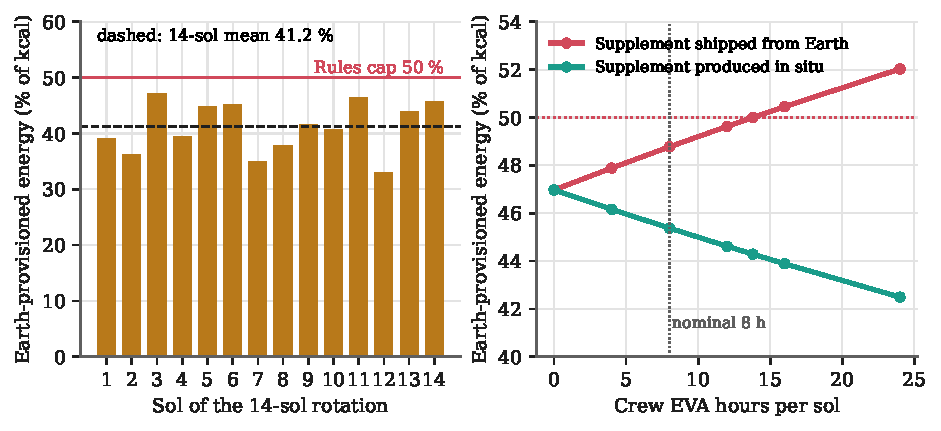
\includegraphics[width=\linewidth]{fig3_earth_fraction.pdf}
\caption{Earth-provisioned share of meal-plan energy. Left: per sol of the 14-sol rotation on the per-ingredient audit (bars), rotation mean 41.2\,\% (dashed) and the 50\,\% rules cap; no sol exceeds the cap. Right: nameplate-basis fraction versus crew EVA hours per sol with the energy supplement shipped from Earth or produced in situ (\cref{tab:eva}); the dotted vertical line marks the nominal 8 crew-EVA-hours per sol.}
\label{fig:earth}
\end{figure}

\subsection{Mass, multi-year operation and maturity}

Launch mass attributable to the food system is \SI{25729}{\kilo\gram}: biological starters \SI{205}{\kilo\gram}, micronutrient premix \SI{180}{\kilo\gram}, allergen-free emergency rations \SI{1500}{\kilo\gram} (90 sols), Earth-provisioned food \SI{6274}{\kilo\gram}, and system hardware, spares and consumables \SI{17570}{\kilo\gram}, of which the six process modules are \SI{2085}{\kilo\gram}. For comparison, fully Earth-supplied food alone for 15 crew over 514 days at \SI{1.8}{\kilo\gram} per person per day is approximately \SI{13878}{\kilo\gram}. The reserve of \SI{4.10e6}{\kilo\calorie} covers 90 sols at full ration or 180 sols at half ration. The programme load over four rotations is approximately \SI{91e6}{\kilo\calorie} ($15 \times 500 \times 3035 \times 4$), 53\,\% met in situ on the nameplate basis. Designed lifetimes are $\geq$\SI{50000}{\hour} for the LED array (about 5.7 years continuous), $\geq$\SI{35000}{\hour} with N+1 redundancy for recirculation pumps, one rotation for hydroponic and photobioreactor membranes, and 12 months for cyanobacterial starter cultures refreshed at each hand-over from Earth cryostock; a 16S rRNA drift assay per rotation triggers refresh at $>2\,\%$ drift.

\Cref{tab:trl} states the technology readiness of each element and the gap to be closed. Overall system maturity is governed by the least mature elements: the regolith classifier at TRL~3, the operations layer at TRL~3--4, and bioremediation and substrate at TRL~4.

\begin{table}[t]
\centering\small
\caption{Technology readiness and gaps.}
\label{tab:trl}
\begin{tabular}{@{}p{3.2cm}cp{4.6cm}p{5.2cm}@{}}
\toprule
Element & TRL & Maturity basis & Gap to close \\
\midrule
Regolith mineral classifier & 3 & Random forest and Gaussian process on published datasets, 77\,\% accuracy; analytical only & Beneficiation hardware; breadboard on simulant before TRL~4 \\
LED sole-source crop production & 6--7 & Veggie and Advanced Plant Habitat heritage \citep{Massa2017veggie}; commercial vertical farming & Fixture lifetime $\geq$\SI{50000}{\hour} under Mars surface conditions \\
Hydroponic staples (wheat, soybean, potato) & 5--6 & Controlled-environment literature \citep{Wheeler2008productivity} & Yield confirmation at \SI{56.5}{\kilo\pascal} \\
Cyanobacterial photobioreactor & 4--5 & Industrial \emph{Arthrospira}; laboratory N$_2$ fixation at low pressure \citep{Verseux2021cyano} & Multi-year culture stability, strain drift \\
Perchlorate bioremediation & 4 & Pathway characterised \citep{Melnyk2011perchlorate} & Rate and completeness in Martian regolith matrix; scale-up \\
Regolith-derived substrate & 4 & Simulant studies \citep{Duri2022regolith} & Validation on in-situ or returned material \\
\emph{Tenebrio molitor} rearing & 5--6 & Commercial industry \citep{vanHuis2013insects} & Closed-loop rearing on in-situ residues; Mars-gravity behaviour \\
Fermentation & 6--7 & Established process control & Starter viability across multi-year storage \\
Operations layer & 3--4 & Component algorithms (scheduling, sensor fusion) established in the literature; the state-inference step was demonstrated on a flight analogue by the author, as a preprint \citep{PuertaAngulo2026hrp} & Closed-loop validation with human subjects in an analogue \\
Surface fission power & 5--6 & KRUSTY demonstration & Outside scope; cited as heritage \\
\bottomrule
\end{tabular}
\end{table}

\section{Discussion}\label{sec:discussion}

\subsection{Principal findings}

Three results carry the argument. First, sizing to crew time rather than to mass or power produces a system in which the two specialists operate at 81--86\,\% of budget on average and 88--90\,\% in the worst window, without overtime, only because two design decisions are load-bearing: the batch-processing galley protocol, which removes 37\,\% of the line-by-line labour, and the all-crew cooking rotation, without which the specialists would require \SI{126}{\hour} per five sols. Neither is hardware. Growing more of a crop is free in power and volume under the rules and expensive in hours; the operations layer exists to buy hours back, not to add capability.

Second, closing the budgets against each other rather than against independent sources is a method with detection power. The withdrawn transpiration figure of \SI{3226}{\litre} per sol was internally plausible (it corresponds to a canopy at DLI 120--130) and was only found to be impossible when checked against the \SI{30.4}{\kilo\watt} of lighting that would have to supply its latent heat. The same coupling fixes the radiator area, the EVA cleaning cadence and, through the \SI{200}{\kilo\calorie} per EVA-hour rule, the calorie budget.

Third, rules compliance on the Earth-provisioned fraction is not a property of the menu alone. Sourced from Earth, the EVA supplement breaches the 50\,\% cap at 13.8 crew-EVA-hours per sol, a variable outside the food system's control; produced in situ, the fraction falls with EVA hours. Where a requirement couples to an external schedule, the compliant design is the one that makes compliance independent of that schedule.

\subsection{Relation to prior closed-system work}

BIOS-3 and Lunar Palace~1 demonstrated multi-month closure of gas and water loops with plant-based food supply for crews of two to four \citep{Gitelson1989bios3,Fu2016lunarpalace}; MELiSSA formalised the compartment model that the present design follows in outline \citep{Lasseur2010melissa}. The present work differs in scale (fifteen crew, \SI{511}{\metre\squared}), in the explicit crew-labour budget, and in the treatment of the Martian atmosphere as a legitimate carbon source: the crew of fifteen supplies only 74\,\% of the carbon fixed by \SI{413}{\metre\squared} of photosynthetic area, and closing that gap from an atmosphere that is 95\,\% CO$_2$ is cheaper than shipping carbon. The photoperiod tessellation is a scheduling result rather than a horticultural one, but it rests on cultivar properties established for controlled environments \citep{Bugbee1997apogee}.

\subsection{The operations layer and human research}

The operations layer proposes per-crewmember portioning from a non-invasive wearable rather than from a laboratory panel, and demotes salivary cortisol from routine sampling to confirmation of a flagged state. That choice rests on two findings from the author's analysis of the SpaceX Inspiration4 public archive (NASA OSDR, $n = 4$, six timepoints) \citep{PuertaAngulo2026hrp}: a fused multi-modal representation separated pre- from post-flight state at leave-one-subject-out accuracy 0.708 against a permuted-label null of $0.489 \pm 0.107$ ($p = 0.026$), whereas no individual biomarker survived multiple-testing correction (0 of 1,112 at Benjamini--Hochberg $q < 0.05$); and eighteen cardiovascular readouts were not distinguishable in classification utility from 406 urine cytokine features at that sample size. The boundary of the claim is stated: the significant result belongs to the fused representation including laboratory modalities, the cardiovascular modality alone was not shown significant, Inspiration4 is a short-duration low-Earth-orbit civilian analogue, and the cited work is a preprint. The layer is therefore specified as a fused state detector whose sampling burden is minimised because sampling is crew time. Routine saliva sampling of fifteen crew at approximately \SI{2.5}{\minute} per sample would cost about \SI{0.63}{\hour} per sol; event-driven confirmation at an assumed two flagged events per five-sol week costs about \SI{0.02}{\hour} per sol. Both durations are engineering assumptions to be confirmed in an analogue campaign.

\subsection{Limitations}\label{sec:limitations}

\begin{enumerate}
\item \emph{No dynamic growth simulation.} Crop yields are taken from a crop table derived from controlled-environment literature; they have not been simulated dynamically nor confirmed at \SI{56.5}{\kilo\pascal}. The carbon ledger inherits this uncertainty.
\item \emph{Crew-time durations are engineering estimates.} The per-ingredient preparation, cooking and cleaning durations were assigned during meal engineering and have not been measured in an analogue galley. The all-crew series and the partition by production method are recomputed here; the non-galley specialist durations (\SI{49.0}{\hour} per cycle) are design allocations and were not recomputed, and the specialists' worst window of 79.5--\SI{81.2}{\hour} is conditional on them.
\item \emph{Energy-audit confidence.} One third of ingredient labels are low-confidence by energy density, although they carry 6.4\,\% of calories. The largest single uncertainty is \emph{Tenebrio} flour at \SI{5.20}{\kilo\calorie\per\gram}, which has no USDA entry and is derived from a declared composition of approximately 50\,\% protein and 30\,\% fat.
\item \emph{Micronutrients.} Values other than macronutrients and sodium are design estimates at 70\,\% yield derating. Iron from whole foods (\SI{20}{\milli\gram} per sol) exceeds the spaceflight ceiling of 8--\SI{10}{\milli\gram} and the rotation as delivered does not meet that requirement. Spirulina and \emph{Tenebrio} flour are the dominant iron sources; reducing their share in favour of soybean products and potato, with ferritin monitoring every 90 sols, is the intended correction and has not yet been applied to the menu.
\item \emph{Maturity.} Three elements are at TRL~3--4. The regolith classifier is trained on published datasets, not on in-situ assay. The operations layer's inference step is demonstrated on a flight analogue but the loop to meal actuation has not been closed with human subjects.
\item \emph{Fixture efficacy.} The 3.0 \si{\micro\mole\per\joule} efficacy is at the favourable end of current commercial fixtures; the installed margin absorbs a 10\,\% shortfall but not more.
\item \emph{Cost and launch architecture.} No cost analysis is presented, and the \SI{25729}{\kilo\gram} launch mass is stated without a delivery manifest.
\item \emph{Evaluation context.} The design was developed for and submitted to a public challenge; it has not been reviewed by an independent engineering board.
\end{enumerate}

\subsection{Future work}

Three activities would move the design most: an analogue galley campaign to measure per-ingredient durations and the WATCH event rate, replacing the engineering estimates of \cref{sec:crewtime-results}; hypobaric yield trials for wheat, soybean and potato at \SI{56.5}{\kilo\pascal} and 21\,\% O$_2$; and in-situ pressing of soybean oil, which at 15\,\% of plan energy is the dominant lever on the Earth-provisioned fraction and would move the audited figure well below 41.2\,\%.

\section{Conclusions}\label{sec:conclusions}

A bioregenerative food system for fifteen crew over a 500-sol Mars surface rotation can be sized so that two food specialists operate within a 45-hour five-sol workweek, provided that galley labour is batched by ingredient event and shared with an all-crew cooking rotation and that monitoring and scheduling are delegated to an operations layer. The system requires \SI{58.1}{\kilo\watt} mean electrical power, \SI{511}{\metre\squared} of growing area and \SI{9.7}{\litre} per sol of make-up water; it fixes more CO$_2$ than the crew produces and returns 116\,\% of the crew's oxygen demand. A 14-sol rotation of 78 distinct meals meets the NASA-STD-3001 energy target with 41.2\,\% of calories from Earth on a per-ingredient audit and 47.0\,\% on a conservative nameplate basis, and producing the EVA supplement in situ keeps that fraction below the cap for any EVA schedule. The reconciliation method---closing lighting, water, heat, gas and crew time against one another---is reported as a result in its own right, because it is how the design's largest error was found.

\section*{Declaration of generative AI in the writing process}
During the preparation of this work the author used a large-language-model assistant for drafting, editing and consistency checking of text and for generating figure and analysis scripts under the author's direction. All design decisions, calculations and their verification are the author's; the author reviewed and edited all content and takes full responsibility for the published article.

\section*{Declaration of competing interest}
The author declares no competing interests.

\section*{Funding}
This work received no external funding.

\section*{Data and code availability}
The delivered 14-sol meal plan workbooks (schedule and lifecycle), the reconciliation scripts (\texttt{01\_recompute\_from\_deliverables.py}, \texttt{02\_figures.py}), their outputs (\texttt{results.json}, \texttt{per\_sol.csv}) and the design documents from which the ledgers are drawn will be deposited at Zenodo \citep{ZenodoEsperanza2026}. The Inspiration4 analysis cited in \cref{sec:discussion} is available at \url{https://github.com/engimine/HRP_Artemis_II} (DOI 10.5281/zenodo.21015202).

\bibliography{references}

\end{document}
